\documentclass[a4paper,12pt]{article}

\usepackage{fontspec}
\setmainfont{CMU Serif}
\setsansfont{CMU Sans Serif}
\setmonofont{CMU Typewriter Text}

\usepackage{polyglossia}
\setmainlanguage{russian}
\setotherlanguage{english}

\usepackage{graphicx}
\usepackage{geometry}
\geometry{left=2.5cm,right=2.5cm,top=2.5cm,bottom=2.5cm}

\usepackage{hyperref}

\usepackage{parskip}
\title{ChessDream : Платформа для Тренеров и Учителей Шахмат}
\author{Габдрахманов Азат}
\date{}

\begin{document}

\maketitle
\tableofcontents
\newpage

\section{Введение}

Chessdream - платформа, обеспечивающая возможность тренеру заключить большую часть тренерской инфраструктуры в одном месте.
Экономия времени. Удобство.

\vspace{0.5cm}
\noindent
\begin{center}
    \textbf{Личный кабинет тренера}
    % \fbox{\parbox[c][5cm][c]{0.8\textwidth}{\centering \Large{Ваше изображение здесь}}}
      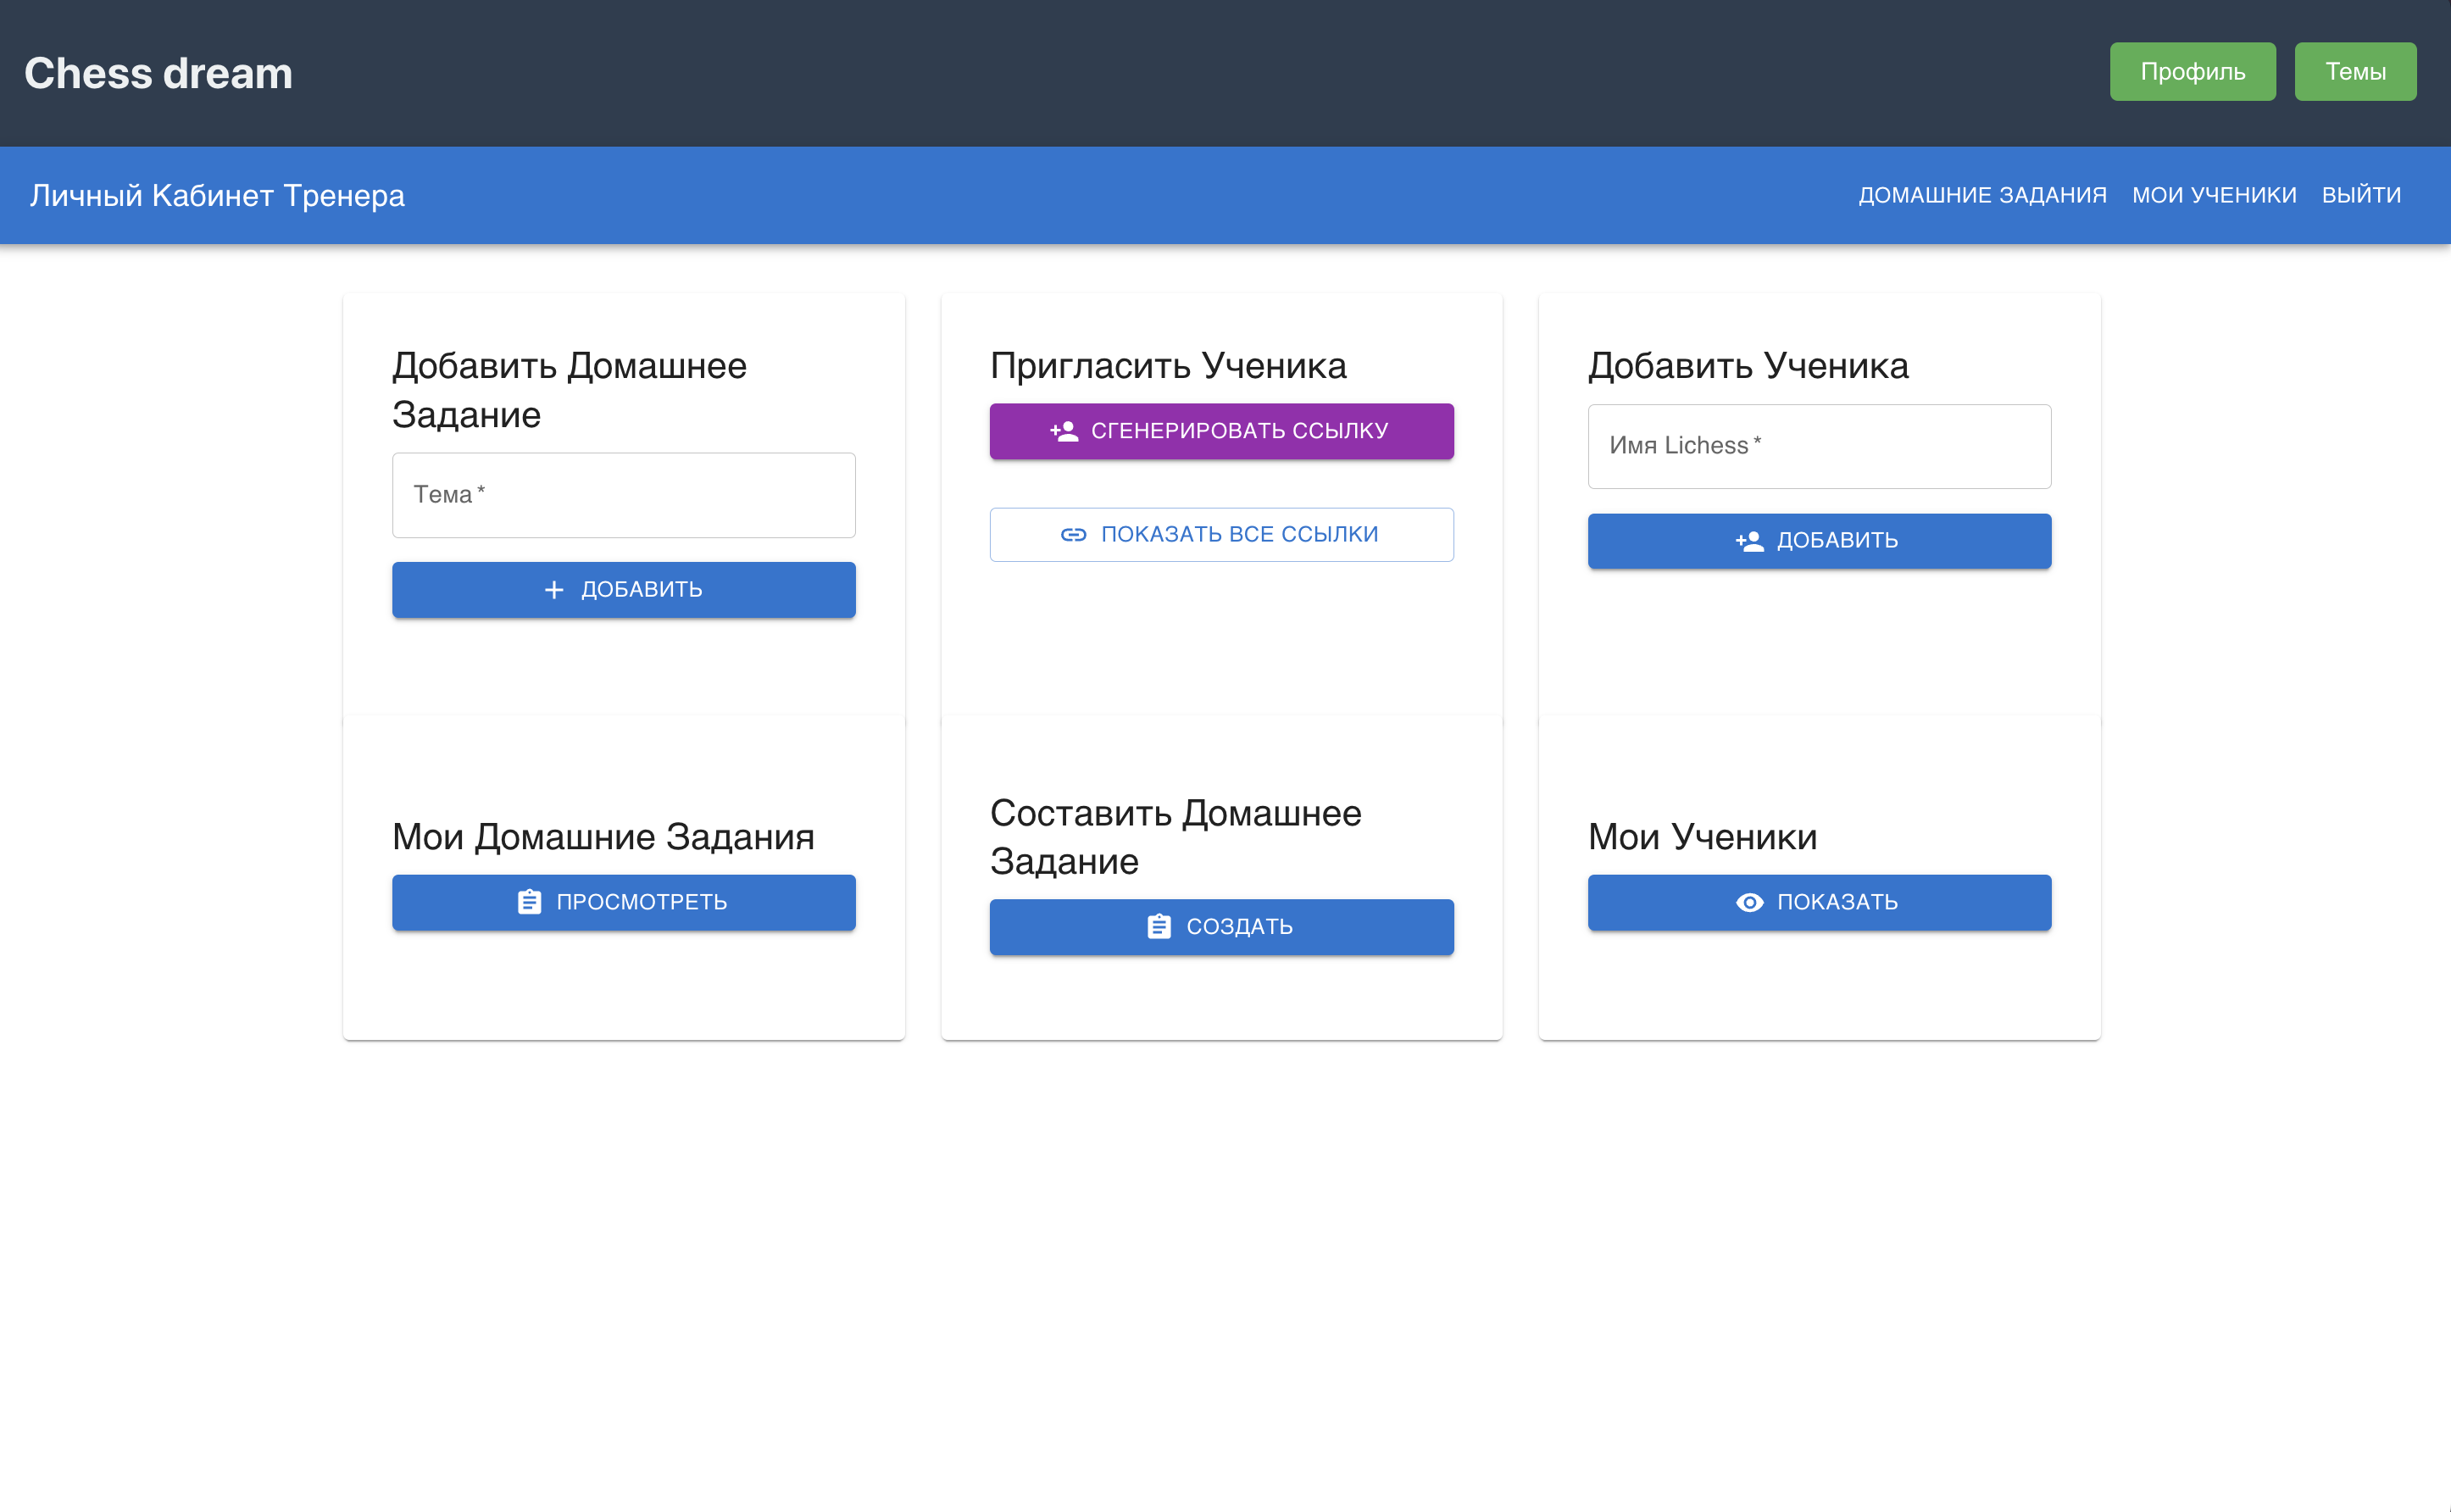
\includegraphics[width=0.8\textwidth]{chessdreampics/coachdashboard.png}
\end{center}
\vspace{0.5cm}

\section{Основная функционалость}

\subsection{Автоматическое формирование домашних заданий}
Наше приложение предлагает решение для автоматизации подготовки домашних заданий. Тренеру достаточно задать параметры:
\begin{itemize}
    \item \textbf{Тема задания. Более 30 тем}
    \item \textbf{Диапазон рейтинга ученика (500-3000).}
    \item \textbf{Желаемое количество задач (от 30 до 100).}
\end{itemize}
Система автоматически подбирает уникальные шахматные задачи из обширной базы данных (база данных аналогична базе данных Lichess), что позволяет избежать повторения и поддерживать интерес учеников.

\vspace{0.5cm}
\noindent
\textbf{Демонстрация генерации задания.}
\begin{center}
    \begin{figure}[htbp]
    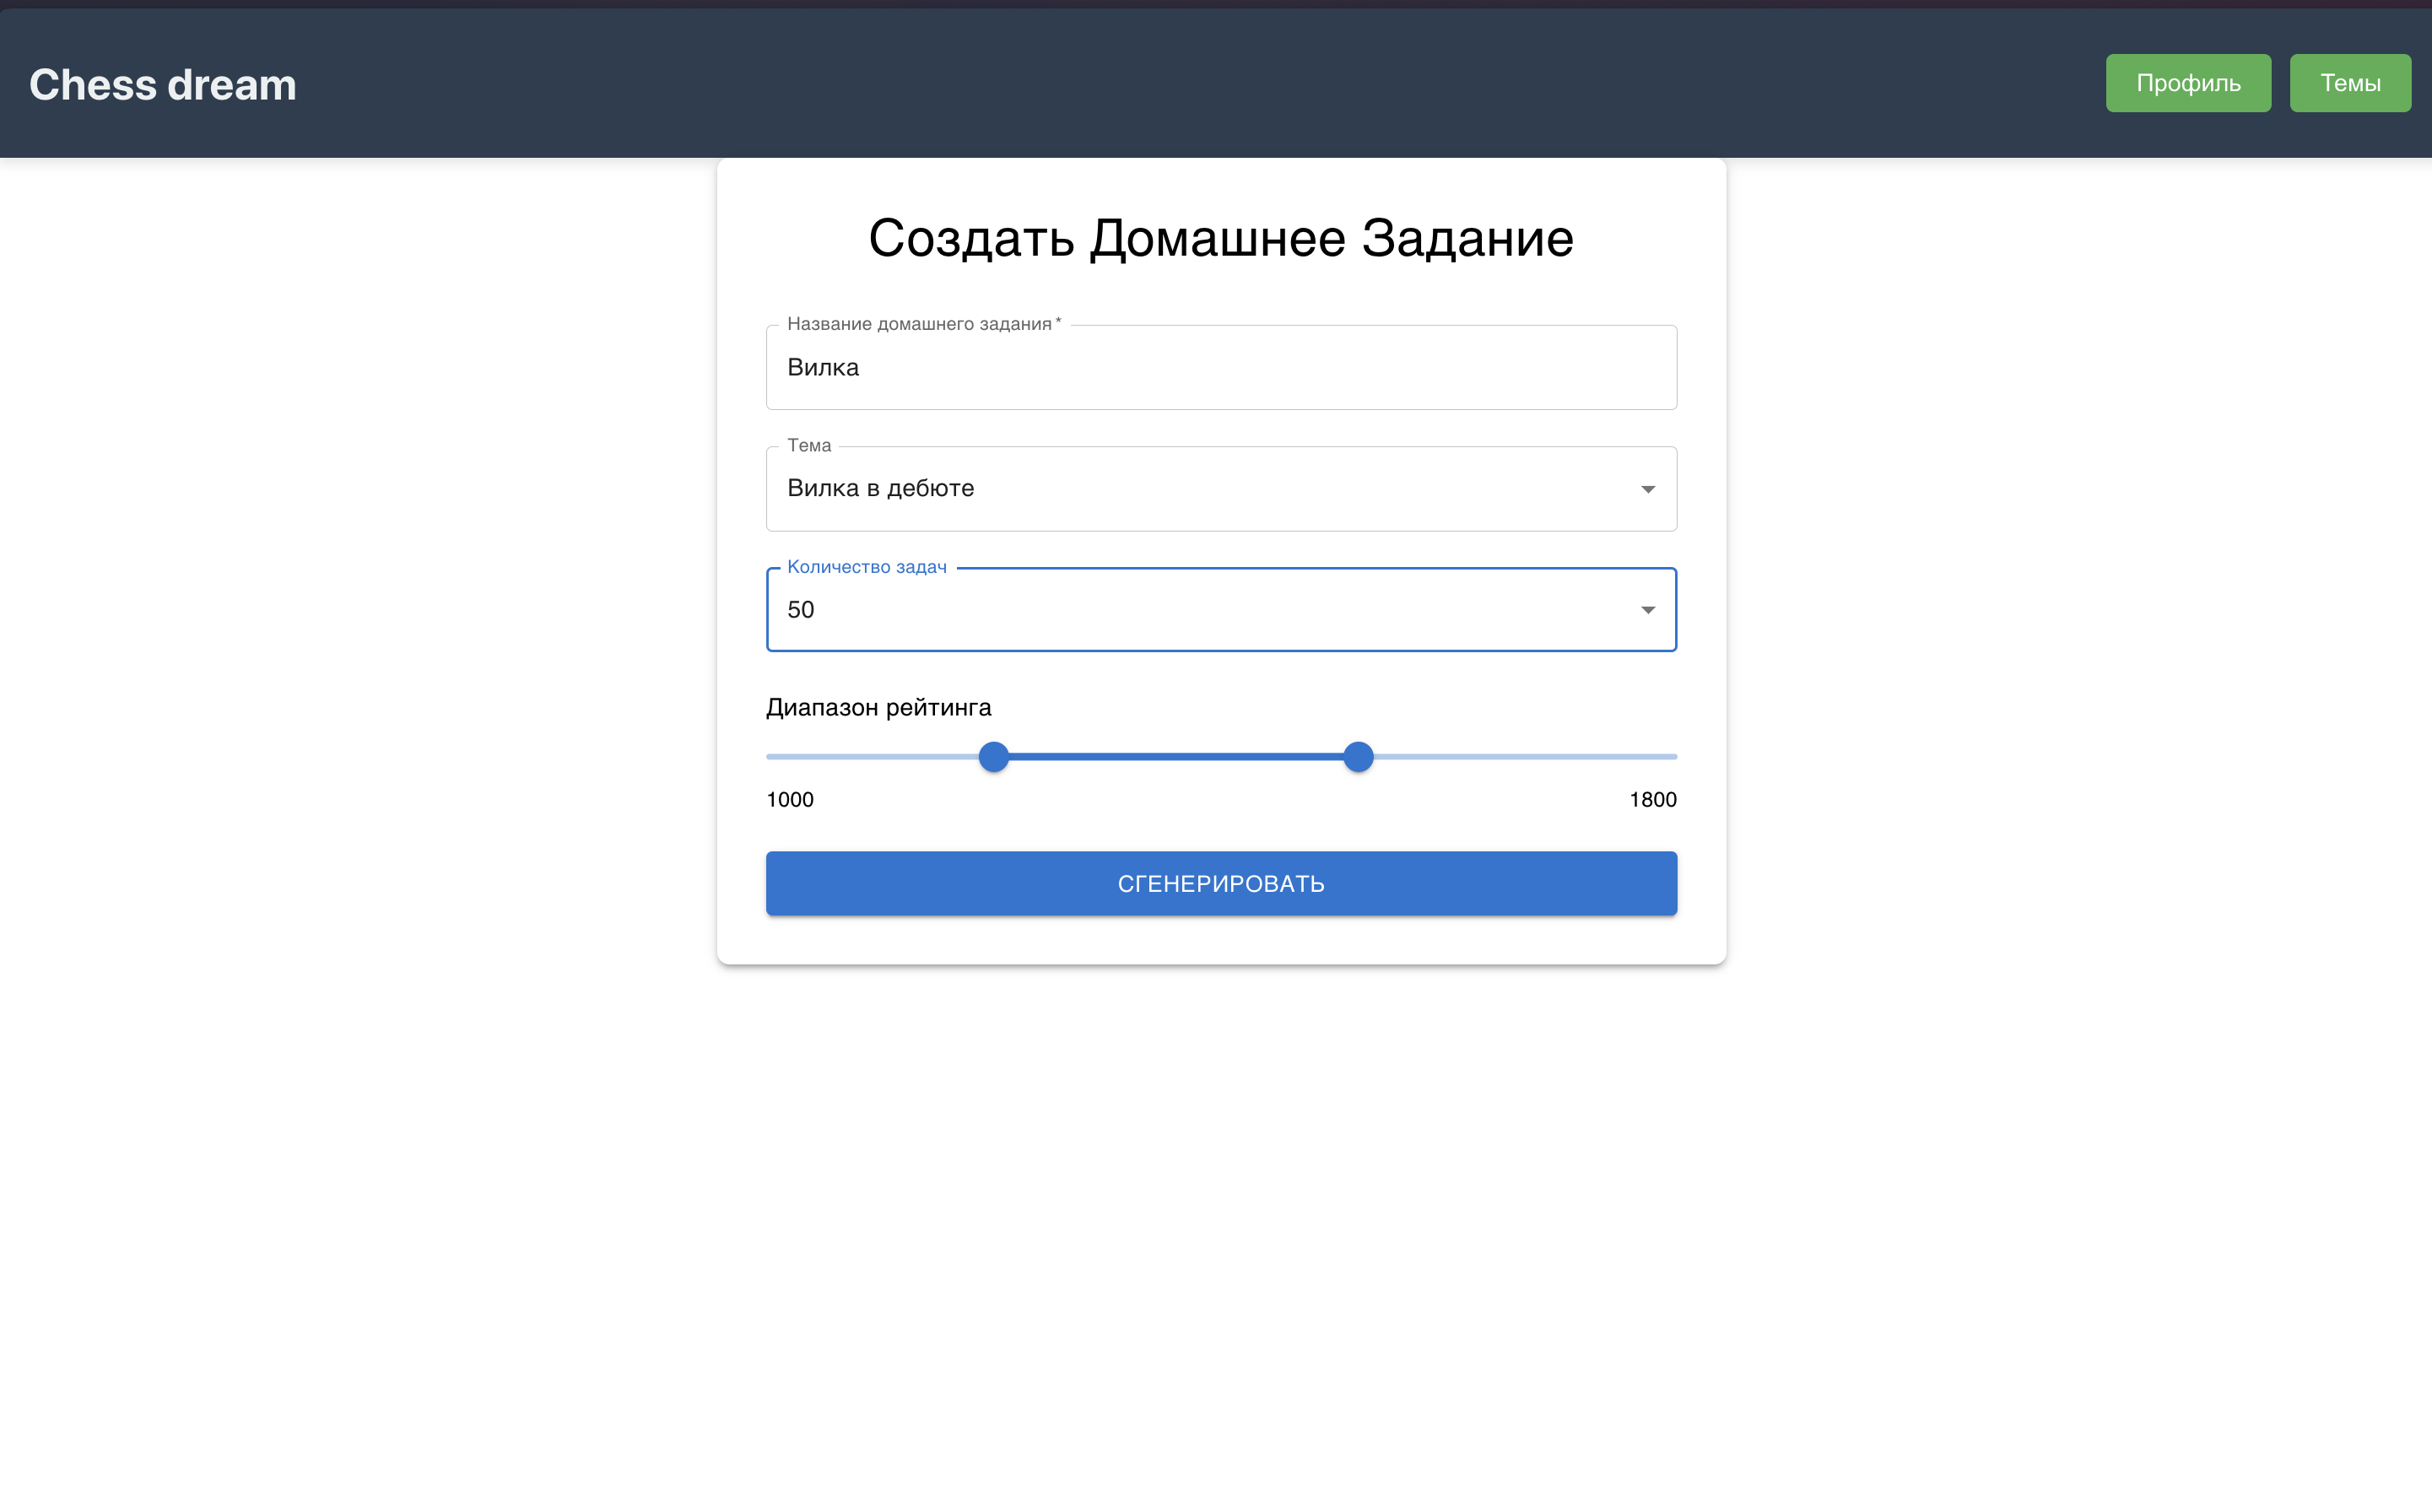
\includegraphics[width=0.8\textwidth]{chessdreampics/homeworkGen.png}
    \caption{Интерфейс для генерации домашнего задания.}
    \end{figure}
\end{center}
\begin{center}
    \begin{figure}[htbp]
    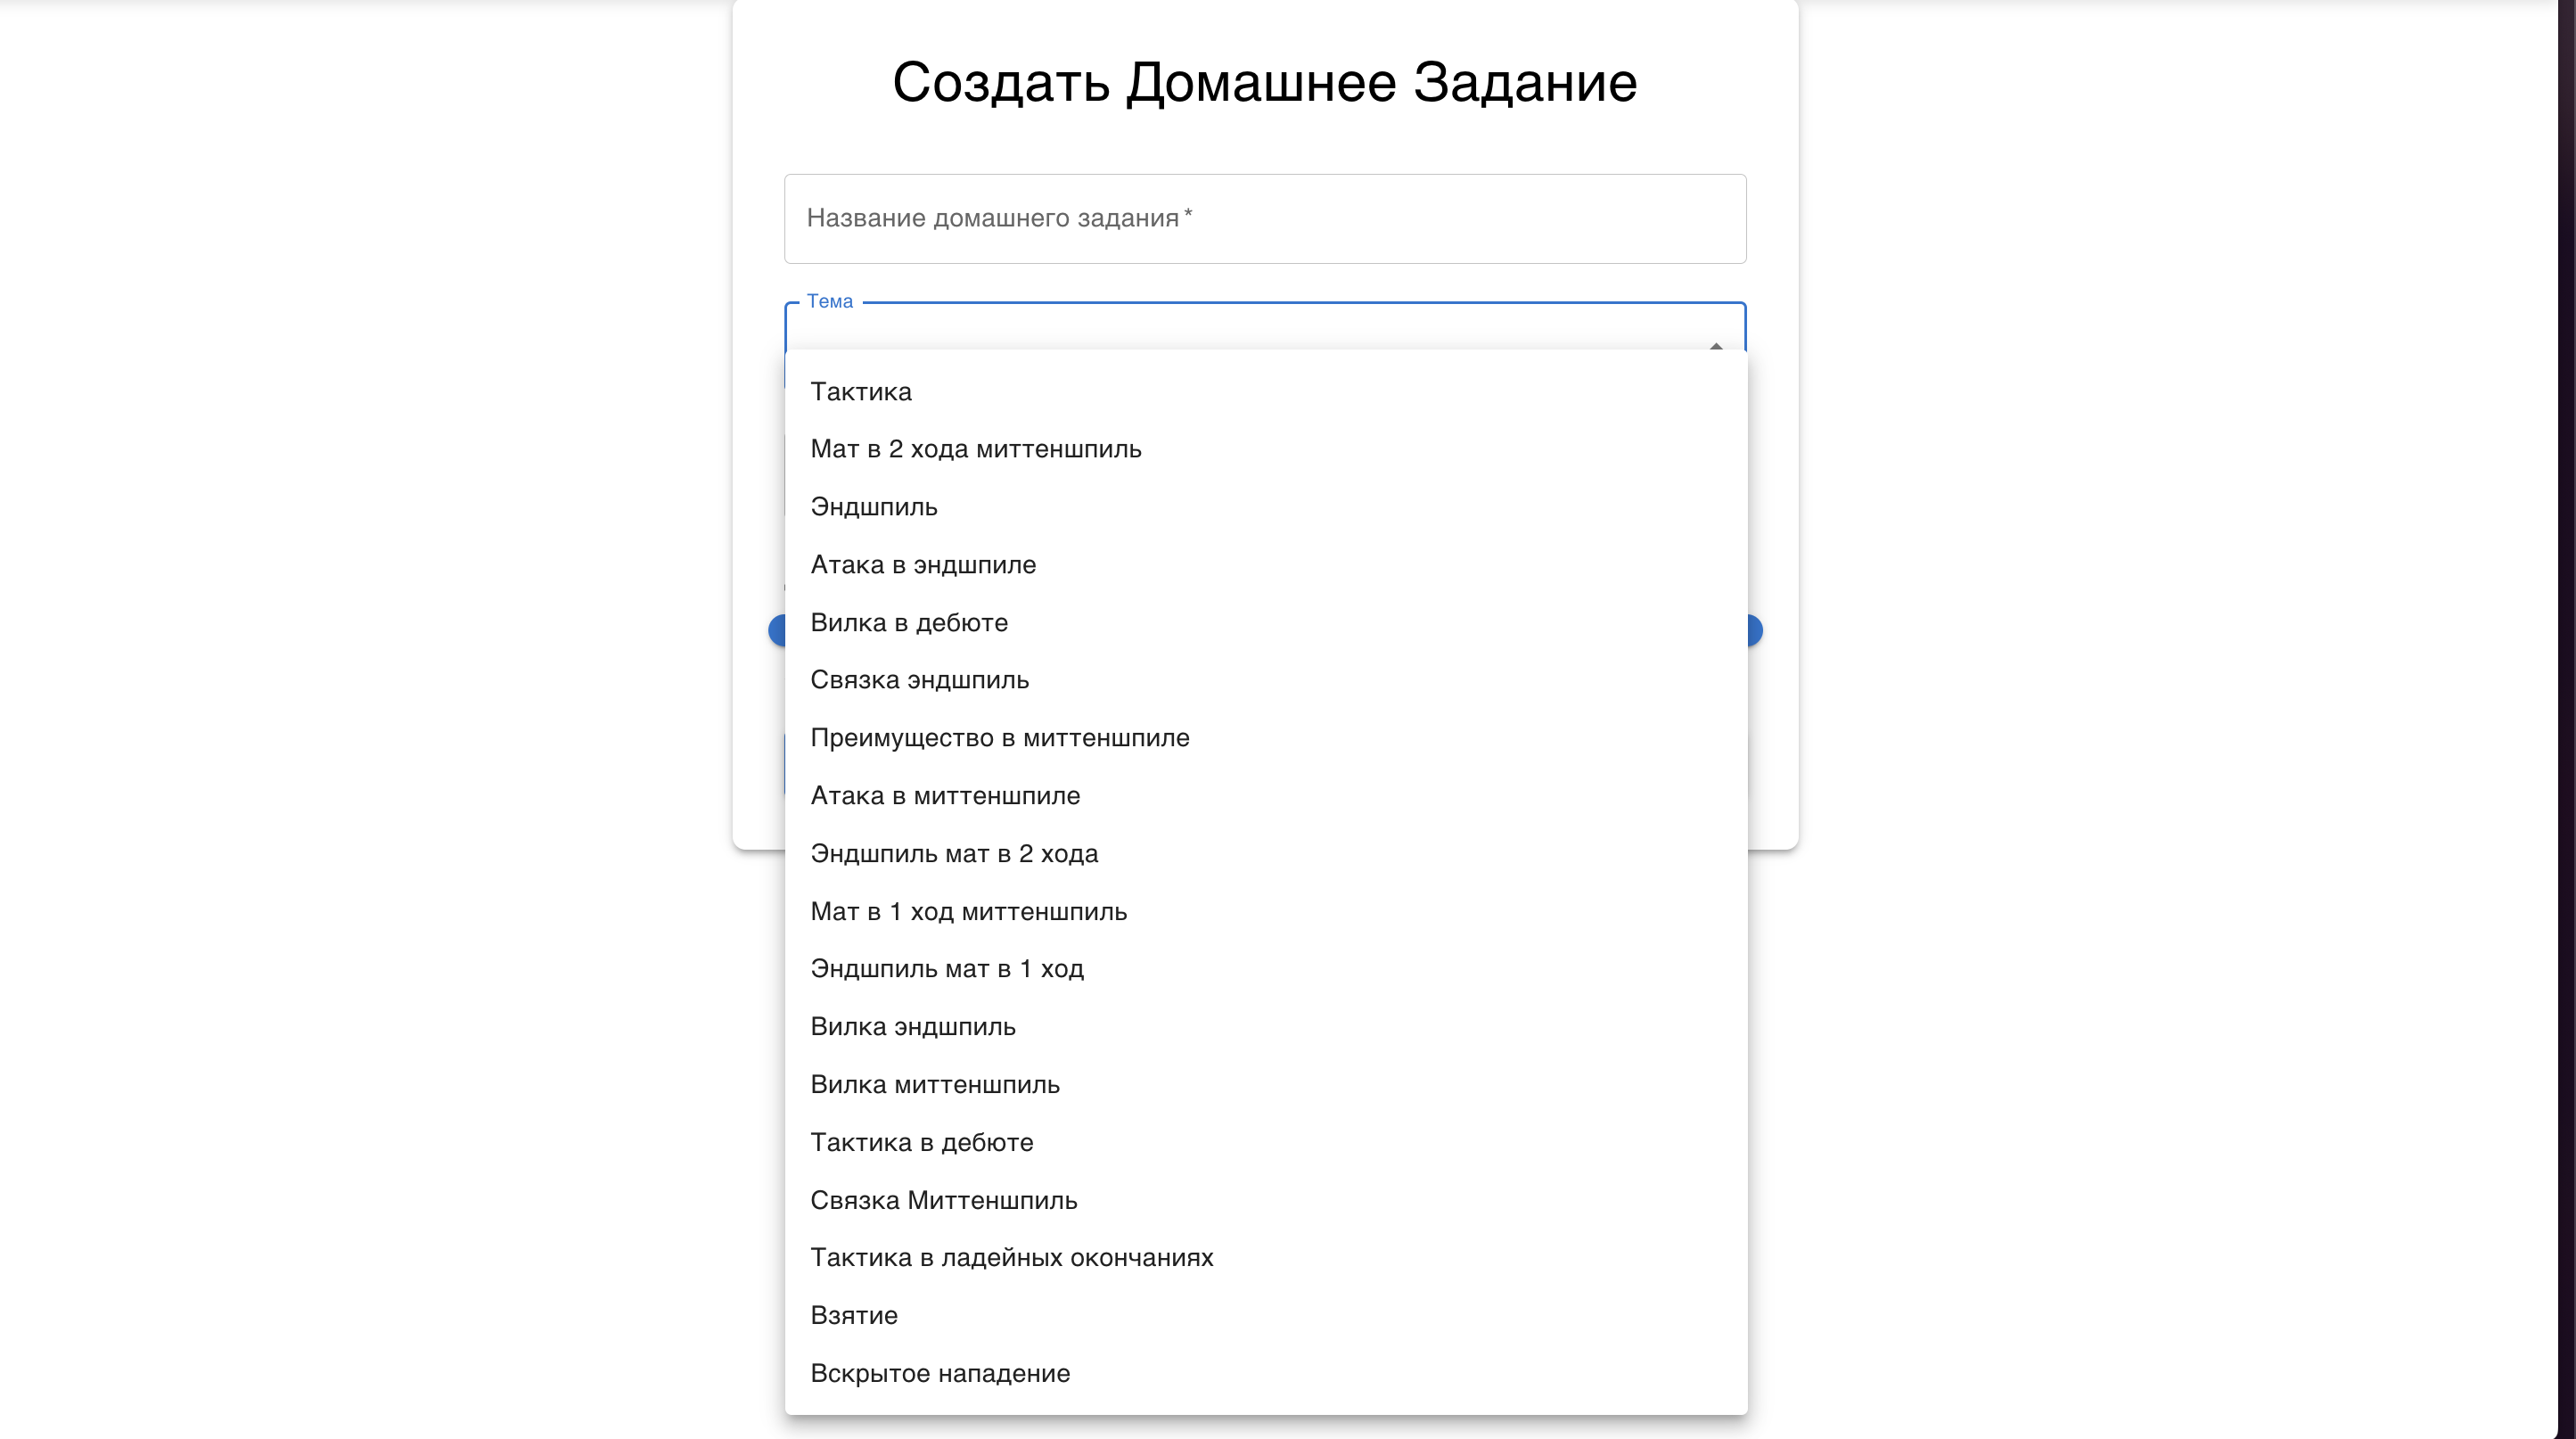
\includegraphics[width=0.8\textwidth]{chessdreampics/themes.png}
    \caption{Возможные темы. (список будет расширяться)}
    \end{figure}
\end{center}
\begin{center}
    \begin{figure}[htbp]
    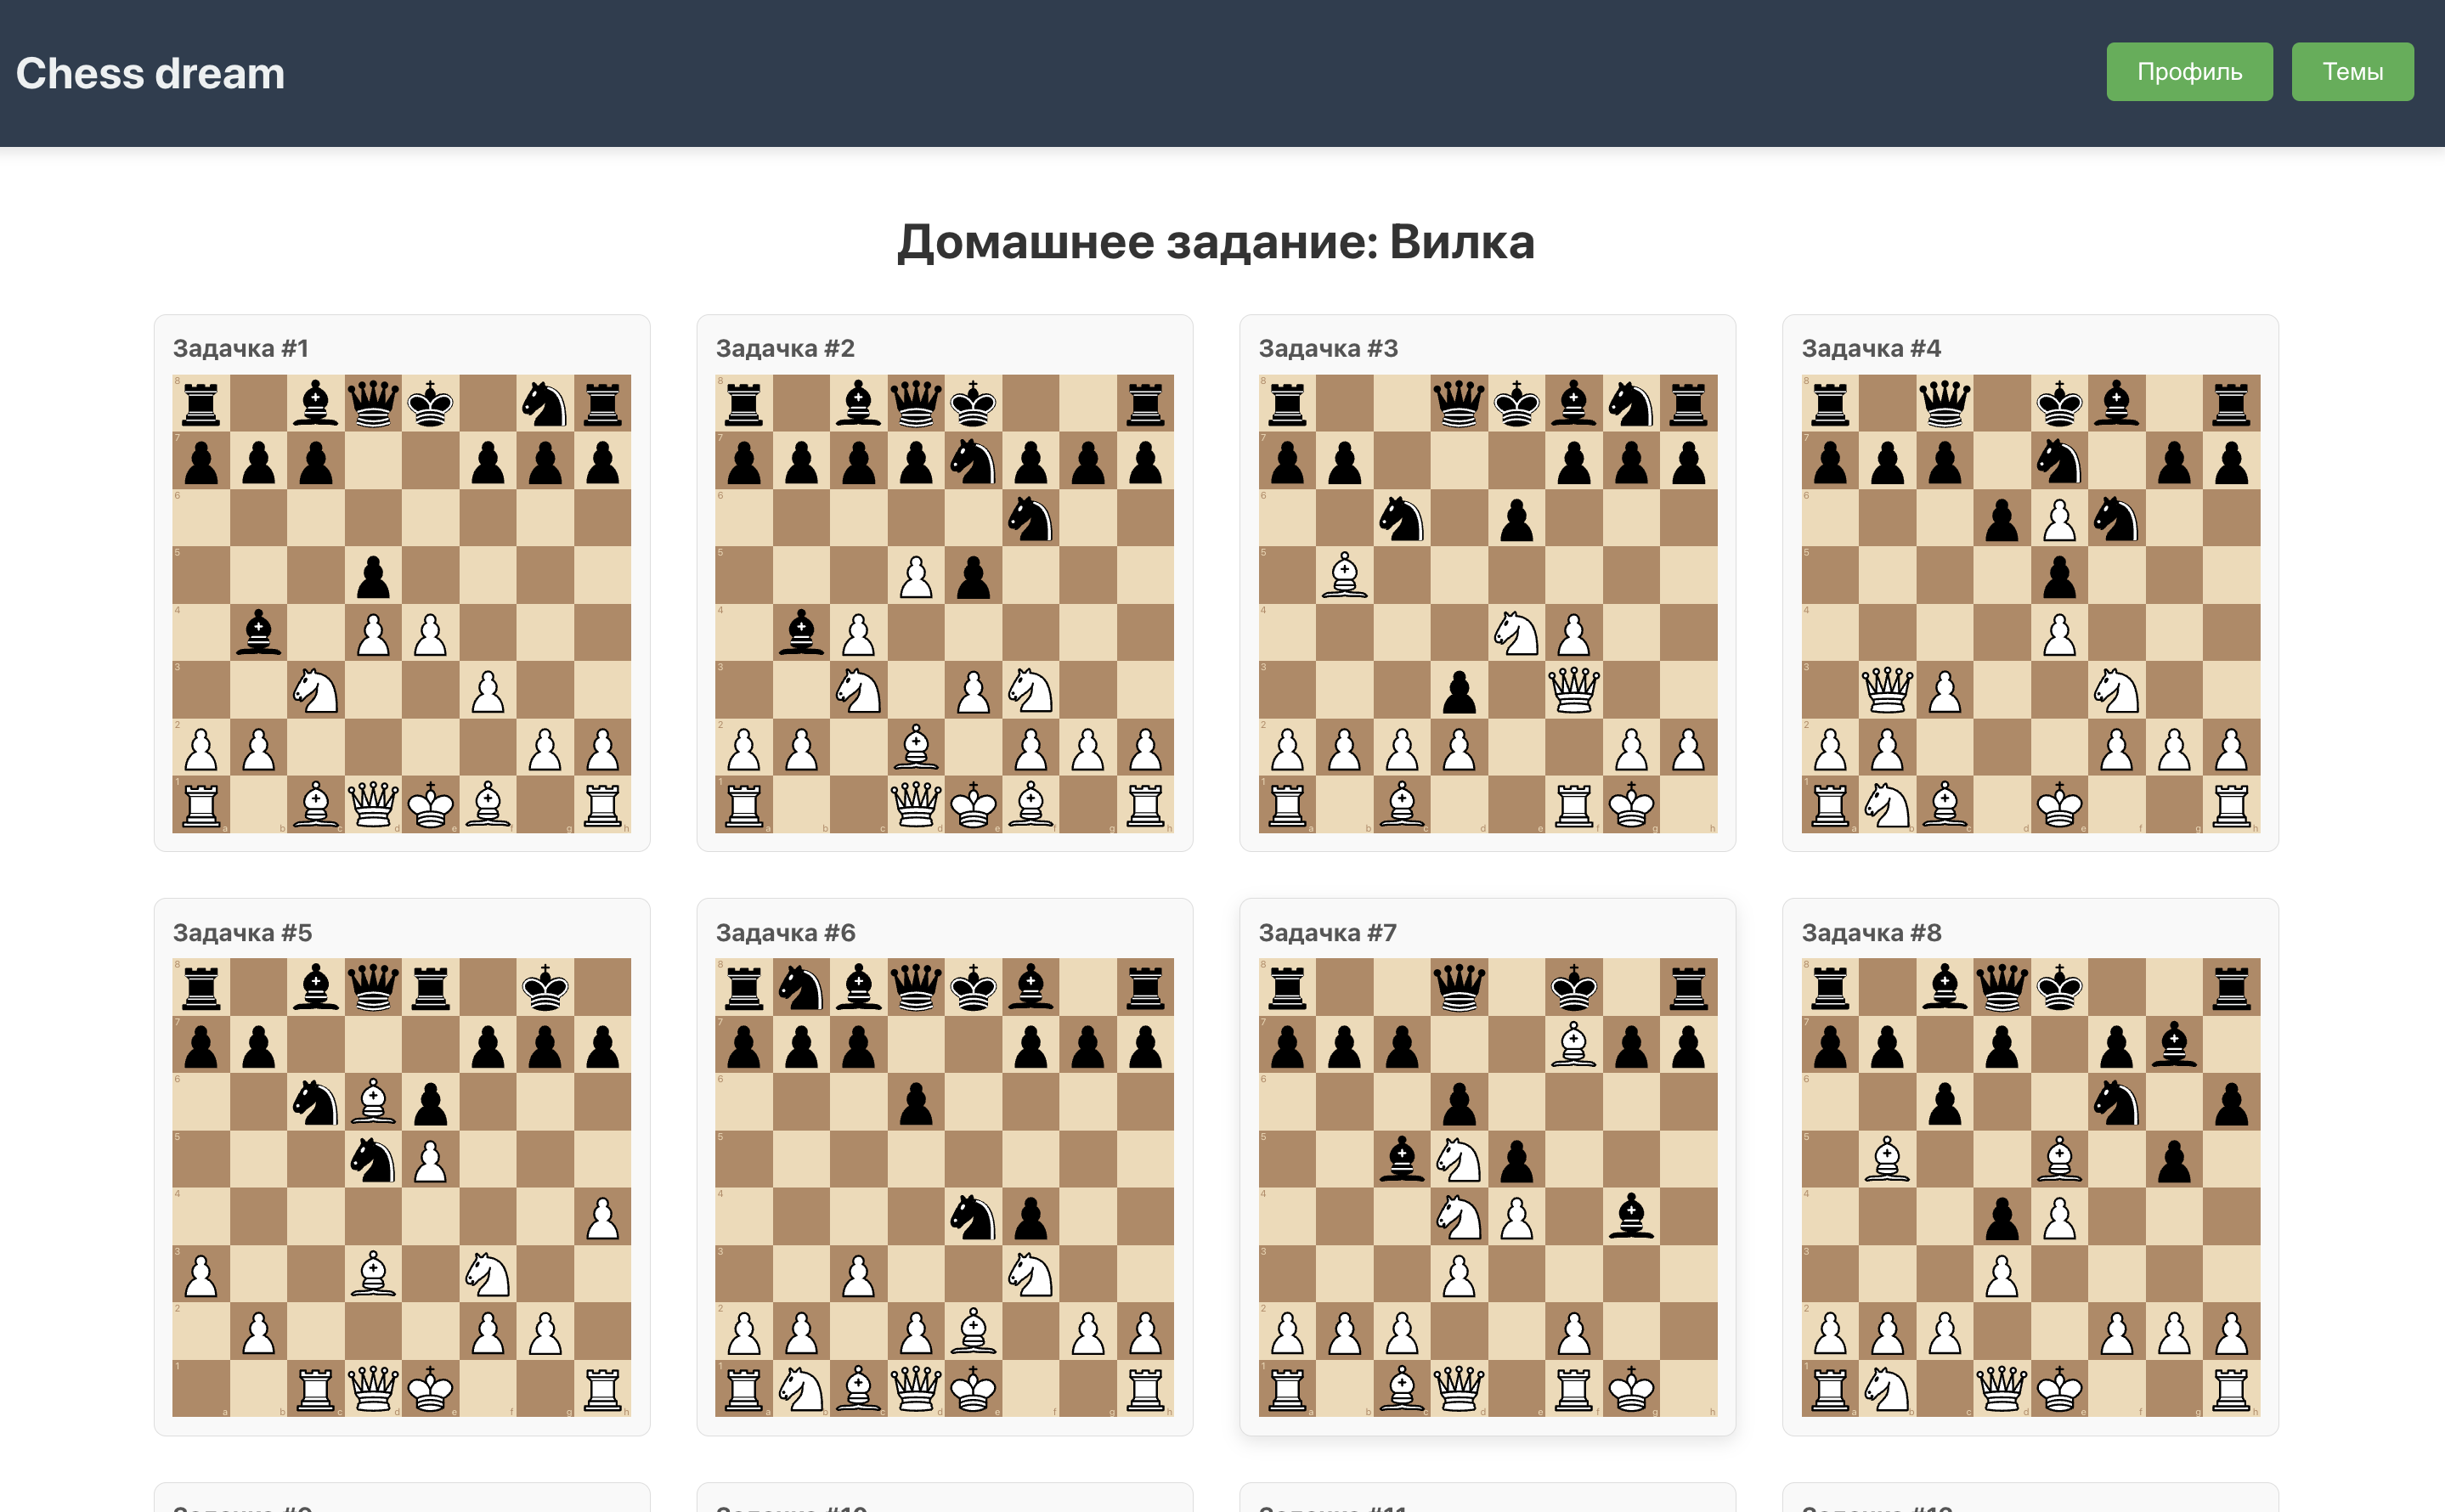
\includegraphics[width=0.8\textwidth]{chessdreampics/homework.png}
    \caption{Сгенерированное дз}
    \end{figure}

\end{center}
\vspace{0.5cm}

\subsection{Контроль выполнения и аналитика результатов}

Платформа не просто выдает задания --- она обеспечивает глубокий анализ каждого выполненного упражнения:
\begin{itemize}
    \item Фиксируется \textbf{время}, затраченное на решение каждой задачи.
    \item Регистрируются \textbf{сделанные ходы} и \textbf{количество допущенных ошибок}.
    \item У тренера есть возможность просмотреть детальную статистику по всему заданию и по отдельной задачке.
    % \item Генерируются подробные \textbf{статистические отчеты}, которые помогают тренеру увидеть динамику прогресса ученика.
\end{itemize}
Эти данные позволяют:
\begin{itemize}
    \item Точно определить слабые и сильные стороны ученика.
    \item Скорректировать план обучения с учетом индивидуальных особенностей.
\end{itemize}

% \vspace{0.5cm}
\noindent
\textbf{Статистика ученика.}
\begin{center}
    \begin{figure}[htbp]
    \includegraphics[width=0.8\textwidth]{chessdreampics/studentprofile.png}
    \caption{Личный кабинет ученика.}
    \end{figure}
    \begin{figure}[htbp]
    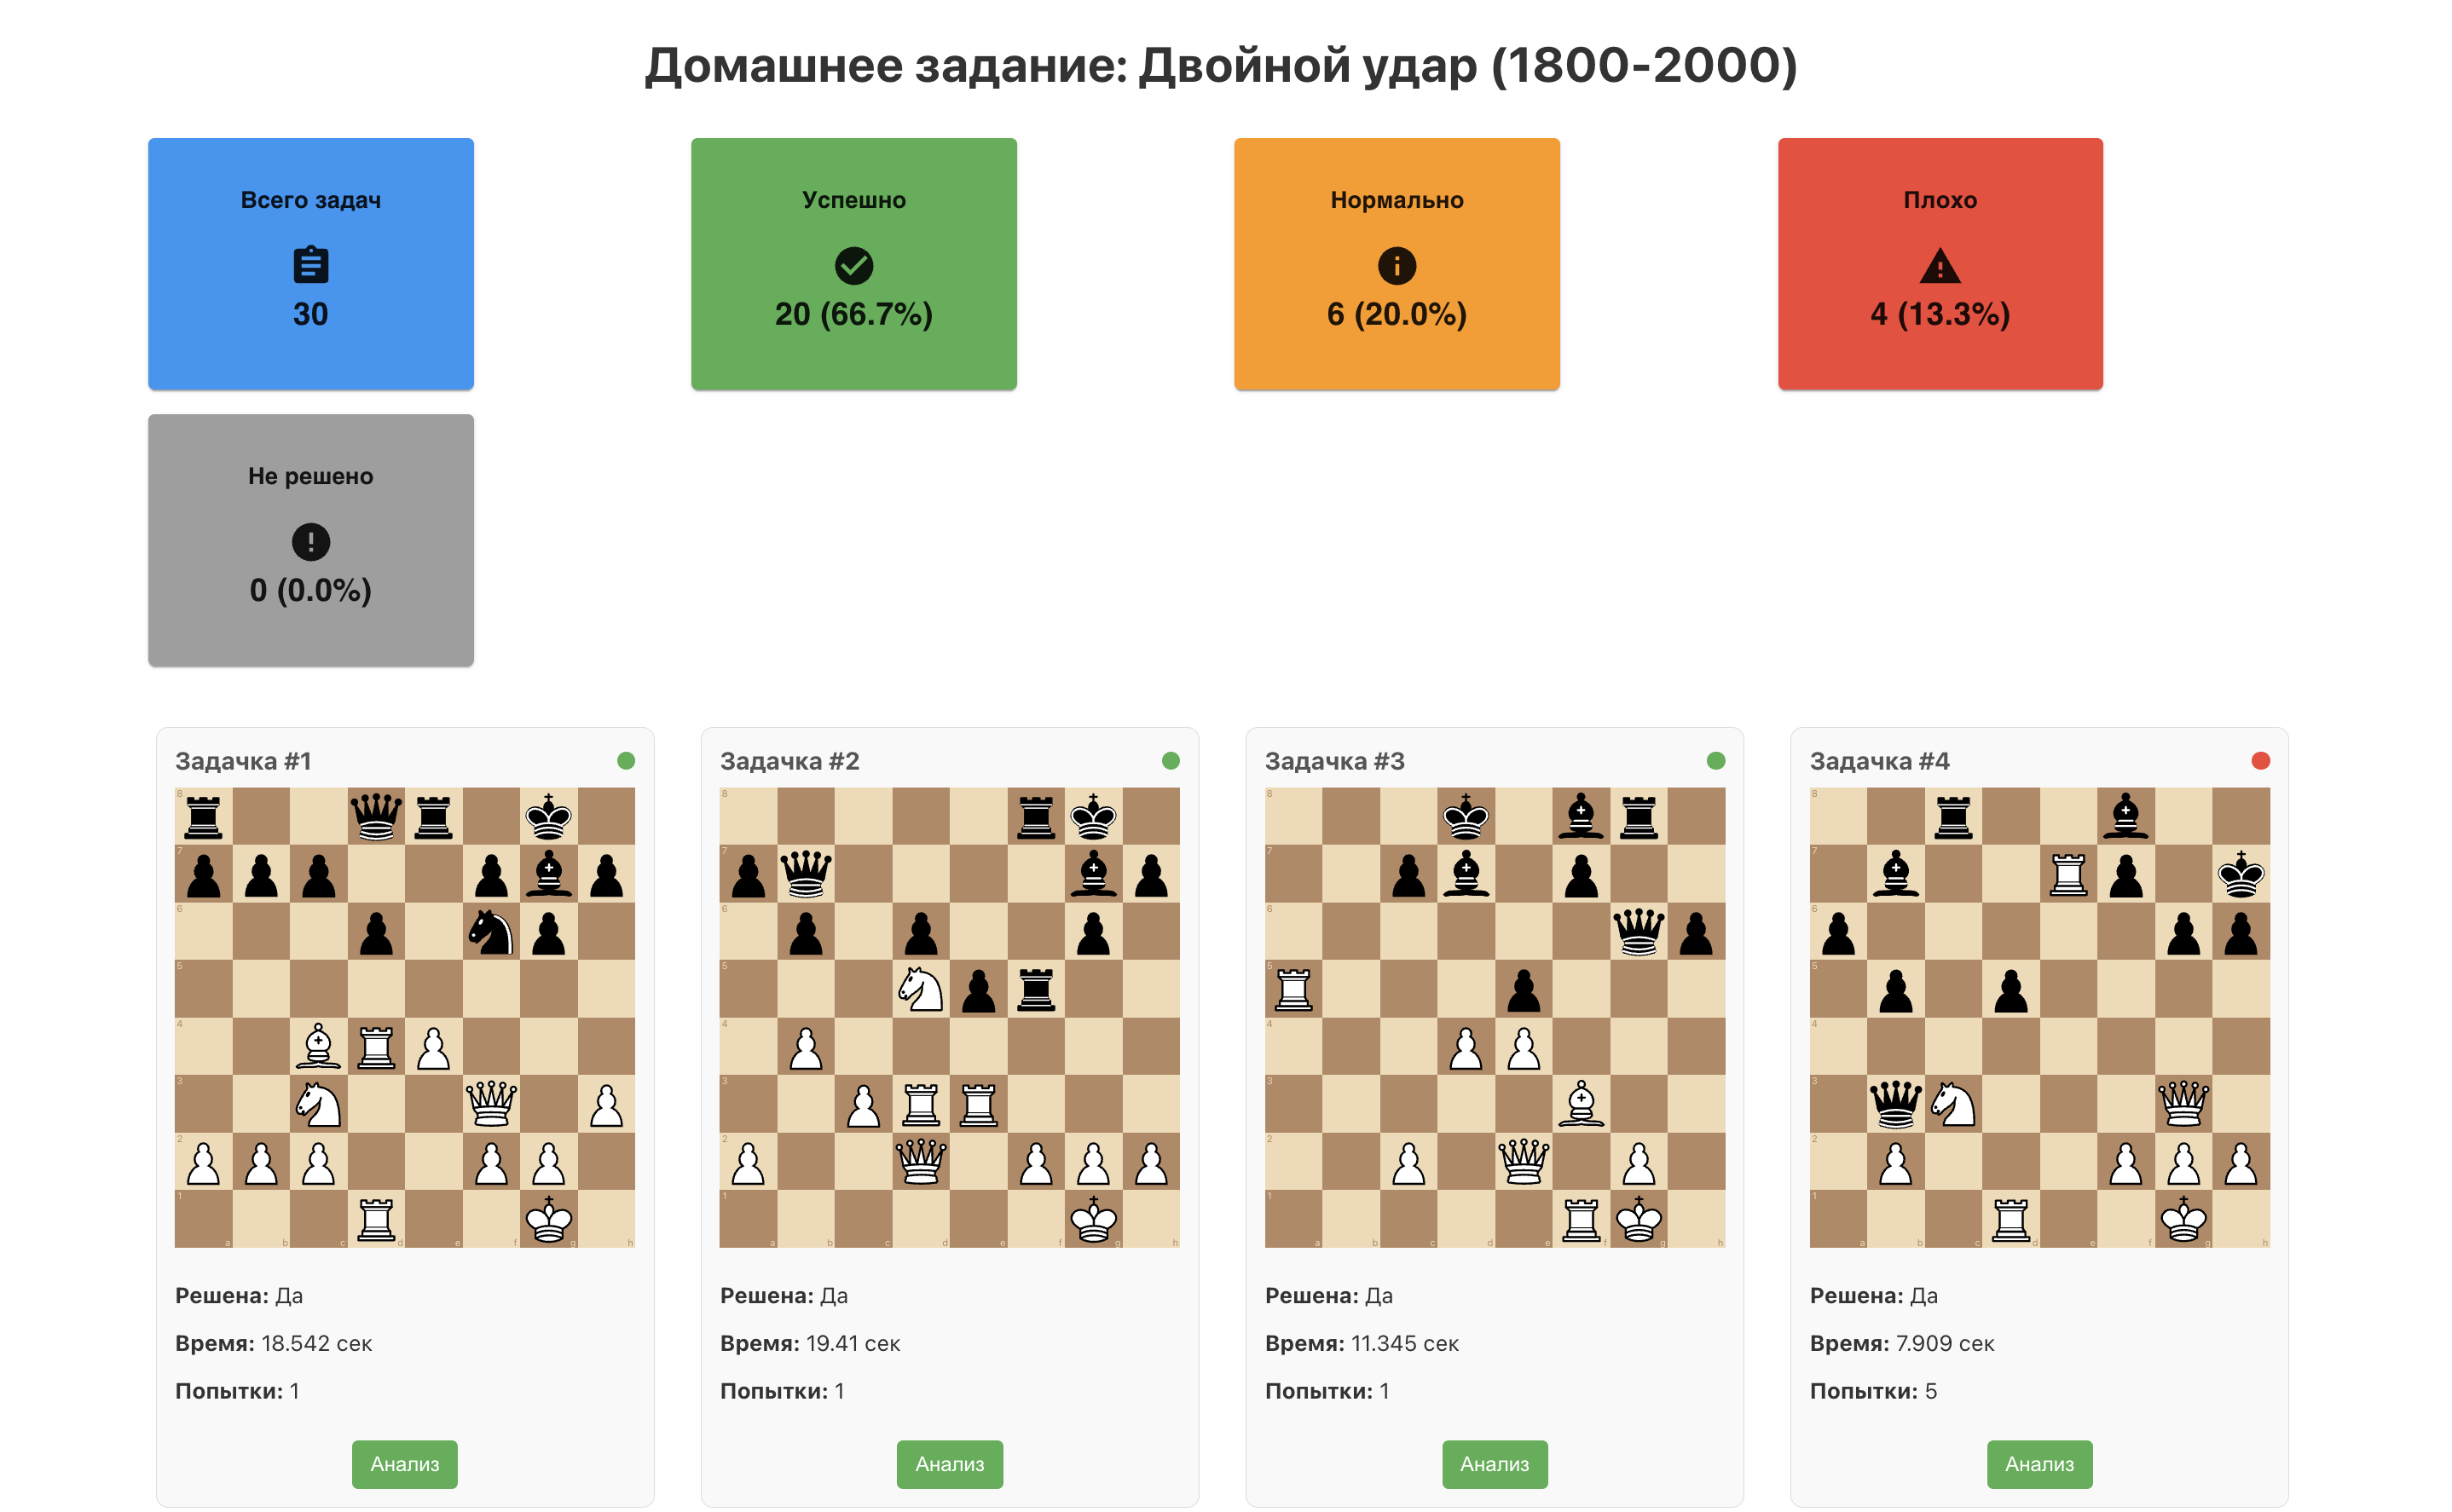
\includegraphics[width=0.8\textwidth]{chessdreampics/homeworkresult.png}
    \caption{Результат домашнего задания ученика.}
    \end{figure}
    \begin{figure}[htbp]
    \includegraphics[width=0.8\textwidth]{chessdreampics/puzzleanalysis.png}
    \caption{Анализ задачки.}
    \end{figure}
\end{center}
\vspace{0.5cm}

\subsection{Персонализированный подход к обучению}
Каждый ученик уникален, и наш продукт ориентирован на индивидуальные потребности:
\begin{itemize}
    % \item Каждое задание адаптируется под уровень и навыки ученика.
    % \item Приложение помогает тренеру выбирать оптимальные задачи, способствующие росту игрока.
    \item Возможность анализа истории выполнения заданий позволяет строить персонализированные планы обучения.
\end{itemize}

\section{Технологические преимущества и безопасность}

\subsection{Современные технологии для стабильной работы}
Наше решение построено на основе клиент-серверной архитектуры, что обеспечивает:
\begin{itemize}
    \item Высокую скорость работы и надежность.
    \item Гибкость в масштабировании для работы с большим количеством пользователей.
\end{itemize}

\subsection{Безопасность и защита данных}
Безопасность --- один из важнейших аспектов нашего проекта:
\begin{itemize}
    \item Использование современных методов шифрования и протоколов для авторизации.
    \item Интеграция с проверенными шахматными сервисами посредством OAuth2.
\end{itemize}
Эти меры гарантируют защиту личных данных тренеров и учеников, а также стабильную работу системы.

% \vspace{0.5cm}
% \noindent
% \textbf{Место для изображения: схема архитектуры системы или блок-схема безопасности.}
% \begin{center}
%     \fbox{\parbox[c][5cm][c]{0.8\textwidth}{\centering \Large{Ваше изображение здесь}}}
% \end{center}
% \vspace{0.5cm}

\section{Преимущества платформы для тренеров и учеников}

\subsection{Преимущества для тренеров}
\begin{itemize}
    \item \textbf{Экономия времени:} Автоматизированное формирование домашних заданий снижает нагрузку на тренера, позволяя сосредоточиться на индивидуальной работе с учениками.
    \item \textbf{Глубокий анализ:} Детальная статистика по выполнению заданий помогает увидеть прогресс и выявить области, требующие дополнительного внимания.
    % \item \textbf{Удобство управления:} Интуитивно понятный интерфейс и удобные инструменты для управления расписанием и заданиями делают процесс обучения эффективным и современным.
\end{itemize}

\subsection{Преимущества для учеников}
\begin{itemize}
    \item \textbf{Адаптированные задания:} Индивидуально подобранные упражнения позволяют постепенно повышать уровень сложности и устранять слабые стороны.
    \item \textbf{Мотивация и развитие:} Постоянная обратная связь и видимый прогресс стимулируют учеников к дальнейшему совершенствованию.
    % \item \textbf{Удобный формат обучения:} Интерактивный интерфейс делает обучение интересным и захватывающим, способствуя росту шахматного мастерства.
\end{itemize}

% \section{Будущие возможности и перспективы развития}

% Мы не останавливаемся на достигнутом и планируем дальнейшее расширение функционала платформы:
% \begin{itemize}
%     \item \textbf{Загрузка и анализ шахматных файлов:} В будущем вы сможете загружать полные партии для подробного анализа, что станет уникальной функцией в сфере шахматного обучения.
%     \item \textbf{Расширение базы задач:} Постоянное обновление и расширение базы шахматных упражнений позволит тренерам всегда находить свежие и интересные задания.
%     \item \textbf{Интеграция с дополнительными платформами:} Планируется расширение функционала за счёт интеграции с другими популярными шахматными сервисами, что сделает процесс обучения ещё более гибким и адаптированным к современным требованиям.
% \end{itemize}

% \vspace{0.5cm}
% \noindent
% \textbf{Место для изображения: иллюстрация будущих возможностей или roadmap развития.}
% \begin{center}
%     \fbox{\parbox[c][5cm][c]{0.8\textwidth}{\centering \Large{Ваше изображение здесь}}}
% \end{center}
% \vspace{0.5cm}

% \section{Заключение}

% \textbf{Шахматное Приложение} --- это не просто инструмент для создания домашних заданий, это полноценная платформа для развития шахматного мастерства. Тщательно разработанный функционал, глубокая аналитика и индивидуальный подход к каждому ученику делают нашу систему незаменимым помощником для тренеров и учеников.

% Погружаясь в мир шахматного развития вместе с нами, вы получаете не только удобный инструмент для работы, но и возможность значительно ускорить процесс обучения, сделать его более осмысленным и эффективным. Присоединяйтесь к нам на пути к новым победам!

\vspace{1cm}
\noindent\textbf{Контактная информация:} \\
% Email: \href{mailto:your-email@example.com}{your-email@example.com} \\
tg: @AzaticG
Веб-сайт: \href{https://chessdream.ru}{chessdream.ru}

\end{document}
